% Please make sure you insert your
% data according to the instructions in PoSauthmanual.pdf
\documentclass[a4paper,11pt]{article}
\usepackage{pos}

\title{Optimisation of the CMS tracker endcap pixel detector as a precision luminometer and background monitor at the HL-LHC}
\ShortTitle{Luminosity and beam background measurement using TEPX at HL-LHC}

\author*[a,1]{Ashish Sehrawat}
\note{For the CMS collaboration.}
\affiliation[a]{Universidad de Sonora,\\
  Blvd. Luis Encinas J, Calle Av. Rosales \& Centro, Hermosillo, Mexico}

\emailAdd{ashish.sehrawat@cern.ch}

\abstract{The High Luminosity upgrade of the LHC (HL-LHC) places unprecedented requirements for background monitoring and luminosity measurements. The CMS Tracker Endcap Pixel Detector (TEPX) will be adapted to provide high-precision online measurements of bunch-by-bunch luminosity and beam-induced background. The implementation of dedicated triggering and readout systems, the real-time clustering algorithm on an FPGA and the expected performance are discussed. The innermost ring of the last layer (D4R1) will be operated independently from the rest of TEPX enabling beam monitoring during the LHC ramp and during unqualified beam conditions. The system optimisation and the dedicated timing and trigger infrastructure for D4R1 are also presented.}

\FullConference{%
  *** The European Physical Society Conference on High Energy Physics (EPS-HEP2021), ***\\
  *** 26-30 July 2021 ***\\
  *** Online conference, jointly organized by Universität Hamburg and the research center DESY ***
}

%% \tableofcontents

\begin{document}
\maketitle

\section{THE CMS PHASE II INNER TRACKER}
The High Luminosity (HL) - LHC will increase instantaneous luminosity to an unprecedented value of 7.5 $\times$ $10^{34} \:cm^{-2} s^{-1}$ which corresponds to 200 proton-proton collisions per bunch crossing. The Run 2 CMS tracker will be replaced to handle the extreme radiation environment, resolve nearby particle tracks and operate properly to give a reliable estimate of the instantaneous luminosity for high pileup values. CMS Phase II Inner Tracker will consists of four barrel layers (TBPX), 8 forward disks per side (TFPX) and 4 endcap disks per side of CMS interaction point. Each TEPX disk will comprise of five rings having 20, 28, 36, 44 and 48 modules respectively. TEPX will be used for tracking as well as luminosity measurement. It will have better radiation tolerance, increased granularity, improved two-track separation,
improved estimation of hit rate and statistical precision, extended tracking acceptance |$\eta$| = 4 with Disk 4 Ring 1 (D4R1) operating as an independent luminometer. TEPX will extend from 1750 mm to 2650 mm in longitudinal direction and from 63 mm to 265 mm in radial direction. Hit occupancy per pixel for TEPX will be less than 0.1\% of entire inner tracker occupancy to ensure excellent tracking under high pileup conditions. It will also ensure pixel cluster counting (PCC) method to be linear with pileup which is used for luminosity determination.

\begin{figure}[htb]
  \centering
  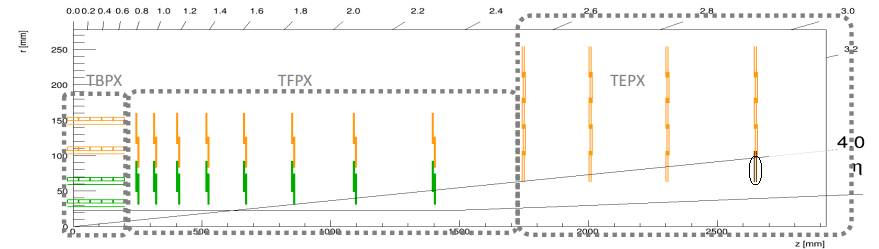
\includegraphics[width=0.8\columnwidth]{tracker_geometry.png}
  \caption{Layout of CMS Phase II Inner Tracker showing Barrel, Forward and Endcap regions. Black circle shows first ring of the last TEPX disk (D4R1).}
  \label{fig:CMS}
\end{figure}


\section{LUMINOSITY MEASUREMENT USING TEPX \& D4R1}
Luminosity measurement requires a luminometer that counts a quantity (hits, clusters, coincidences) linear to number of primary interactions. Luminosity measurement during Phase II will be done using two different systems: TEPX and D4R1. TEPX will be used in physics conditions for tracking but will also get a dedicated trigger generated by the BRIL trigger board, data will only be processed by luminosity hardware of TEPX and send to BRILDAQ. D4R1 will be a dedicated luminometer with dedicated triggers fully independent of the CMS DAQ system for data analysis. Luminosity measurement using TEPX will be based on real time pixel cluster or coincidences counting (PCC) on FPGA, a method which involve counting the number of pixel clusters in the pixel detector (innermost part of the CMS tracker) per bunch crossing in minimum bias events. PCC is used for luminosity measurement because it shows excellent linearity over large pileup range. Clusters are collection of hits created by particle tracks and two fold coincidences are clusters in modules overlapping regions formed by modules in front and back layers of TEPX disk. Luminosity measurement based on counting coincidences has an advantage over clusters that afterglow effects are less in the case of coincidences. The innermost ring of the last disk of TEPX (D4R1) is located at 2.65 m away from the interaction point that is beyond the tracking acceptance (|$\eta$| = 4) and as this region has few tracking points, it can be solely used for the purpose of luminosity measurement by using the full available trigger rate 825kHz (750 kHz +75 kHz) and bandwidth. Expected CMS L1 trigger rate is around 750 kHz at <PU> = 200. 500 kHz trigger rate during Van der Meer scans (<PU> = 0.5) and 75 kHz (10\% of expected CMS L1 trigger rate) trigger rate will be used for TEPX luminosity measurement at <PU> = 200. 1000 kHz trigger rate during van der meer scans (<PU> = 0.5) and 825 kHz trigger rate will be used for D4R1 luminosity measurement at average <PU> = 200.

\begin{figure}[htb]
  \centering
  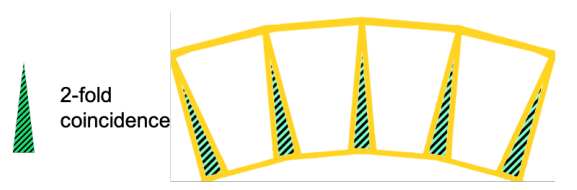
\includegraphics[width=0.6\columnwidth]{twofold1_new.png}
  \caption{Module overlaps in TEPX disk showing two fold coincidences.}
  \label{fig:CMS}
\end{figure}


\section{TEPX \& D4R1 TRIGGER AND TIMING SYSTEM}
TEPX and D4R1 will require BRIL trigger board (BTB) independent of CMS L1 trigger system to have full control over luminosity triggers, local TCDS2-like control stream for D4R1 synchronised to LHC clock, luminosity local L1 triggers and encoding of beam 1 \& beam 2 logical signals. CMS Timing and Control Distribution System (TCDS) receives LHC Clock and Orbit signals that are generated by the LHC RF system and uses them for generating the CMS Clock and commands. Measurement of beam induced background using D4R1 during the LHC ramp will need to be independent but synchronized to the rest of CMS and the central services like TCDS2 and data acquisition will be implemented using special clocking
scheme. Trigger and Timing subsystem for D4R1 will receive a dedicated “TCDS2-like” control stream from the BRIL trigger board (BTB) that is based on the LHC clock.

\begin{figure}[htb]
  \centering
  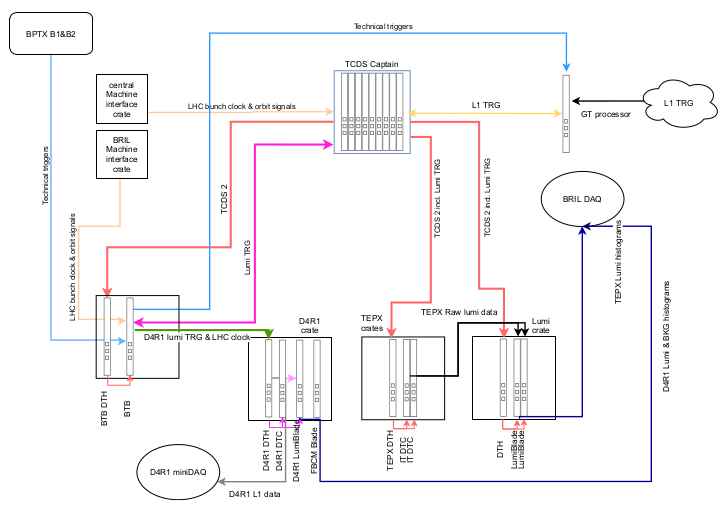
\includegraphics[width=0.4\columnwidth]{BTB.png}
  \caption{Luminosity-centric schematic of the trigger, timing, and data flow in the Phase-2 TEPX system. TEPX will receive luminosity triggers from the BRIL trigger board via central TCDS2, whereas D4R1 will receive a dedicated stream based on the LHC machine clock.}
  \label{fig:CMS}
\end{figure}


\newpage
\section{TEPX FRONT-END AND BACK-END}
Data accepted by CMS L1 trigger (750 kHz) will be collected by the end column of the pixel chip in TEPX and sent through electrical links (eLinks) at 1.28 Gb/s to LpGBT ASICs for optical transmission. Backend system DTC will be connected to frontend TEPX electronics via low-power Gigabit Transceiver (LpGBT) optical links. Optical down-links at 2.5 Gb/s will be used for clock, trigger, commands, and configuration data to the pixel modules. Optical up-links at 10 Gb/s will carry readout data from L1 accept and monitoring information to the DAQ and control system. TEPX luminosity processing will be performed by a separate luminosity processor board to which the DTC backend will send data over ~4 $\times$ 25 Gb/s optical links.


\begin{figure}[htb]
  \centering
  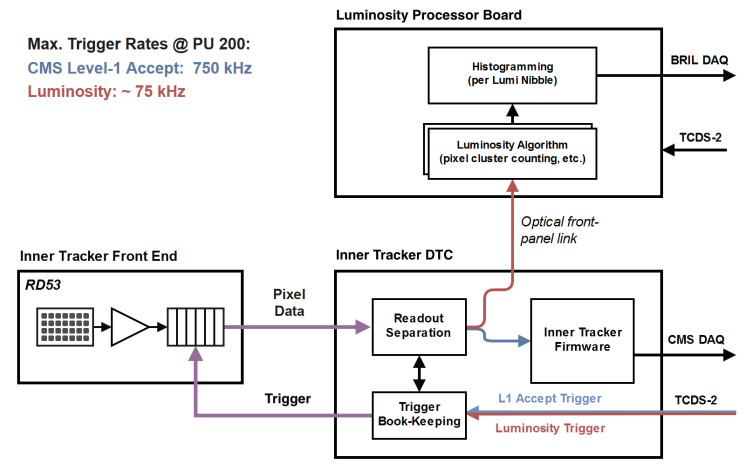
\includegraphics[width=0.5\columnwidth]{TEPX_dataflow.png}
  \caption{Data flow for CMS Phase II Inner Tracker used for luminosity measurement. }
  \label{fig:CMS}
\end{figure}


\section{TEPX CLUSTERING ALGORITHM}
TEPX luminosity processing FPGA will consist of pixel clustering and histogramming instances. Clustering firmware will consist of
Stream decoder that will receive TEPX chip data, separate it from data appended by DTC and decode it. Quarter core processor will be used to identify up to four possible clusters within a quarter core. Two hits form a cluster if they touch horizontally, vertically or diagonally. Quarter core distributor will check a given quarter core for isolation and decides whether it has to be sent to the row merger or counted internally. Count accumulator will receive final data bit and increment cluster count.\\


\begin{figure}[htb]
  \centering
  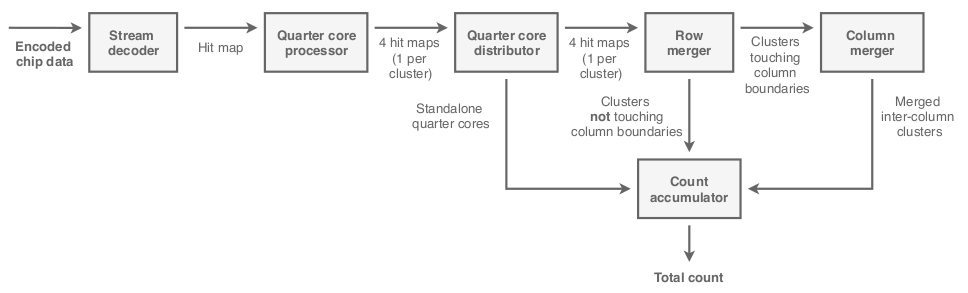
\includegraphics[width=0.6\columnwidth]{CA.png}
  \caption{ TEPX clustering firmware.}
  \label{fig:CMS}
\end{figure}

A prototype pixel cluster counting algorithm has already been developed on FPGA board by injecting CMSSW TEPX events at 1000 kHz event rate. Mismatch cluster count is 0.021\% because offline PCC algorithm applies two thresholds (charge and size of cluster) to the hit data.
Measured maximum event rate is $f_{max}$ = 1.33 +- 0.44 MHz at <PU> = 200 which satisfies D4R1 requirements.


\section{TEPX \& D4R1 EXPECTED PERFORMANCE}
Simulated data samples for Phase II were produced including full CMS detector description and using official CMS software (CMSSW) that calls GEANT4 for particle and energy deposit simulation as well as for reconstruction. Samples contain single-neutrino event overlaid with a variable number of minimum-bias events (events with any amount of real energy detected in CMS) to simulate different pileup values. Linearity for TEPX and D4R1 luminometer is expected to be within 1\% over entire pileup range. Statistical precision is an important uncertainty that need to be considered for precise luminosity measurement that is calculated by taking product of cluster or coincidence counts per collision event, trigger frequency and time integration period. Expected statistical precision for TEPX and D4R1 luminometer is around 0.1\%


\begin{figure}[htb]
  \centering
  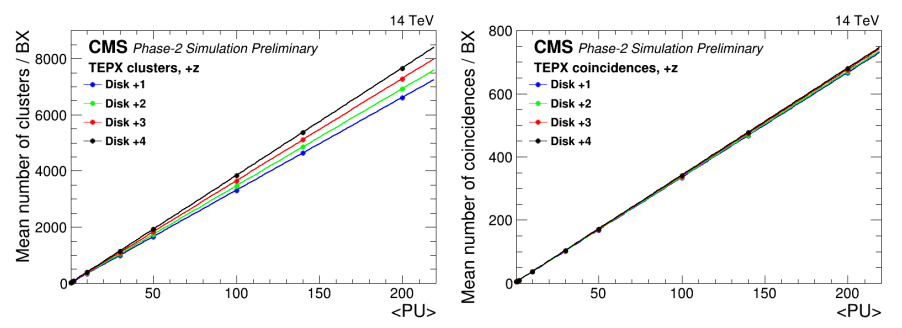
\includegraphics[width=0.6\columnwidth]{SP4.png}
  \caption{Left: Simulated mean number of clusters for TEPX disks as a function of pileup. Right: Simulated mean number of coincidences for TEPX disks as a function of pileup.}
  \label{fig:CMS}
\end{figure}


\begin{figure}[htb]
  \centering
  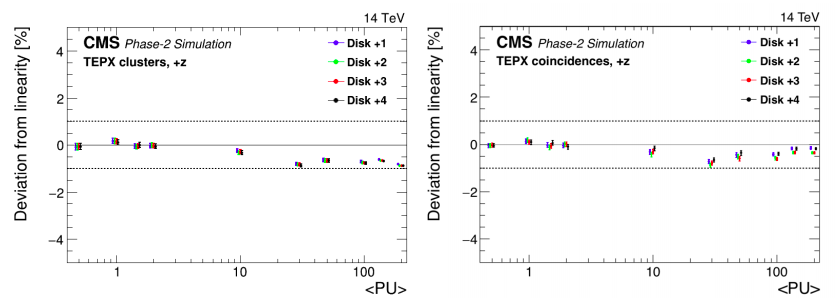
\includegraphics[width=0.6\columnwidth]{residuals_new.png}
  \caption{Left: Cluster non-linearity is within 1 \% for entire pileup range. Right: Coincidences non-linearity is within 1 \% for entire pileup range. }
  \label{fig:CMS}
\end{figure}


\begin{table}[htb]
  \centering
   \caption{ Expected statistical precision for different TEPX disks and rings.}
  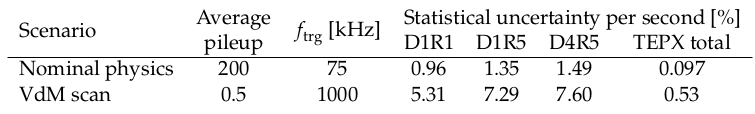
\includegraphics[width=0.6\columnwidth]{SP2.png}
  \label{Table:CMS}
\end{table}

\begin{figure}[htb]
  \centering
  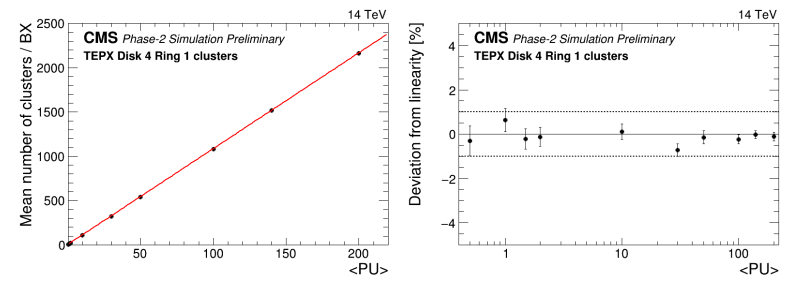
\includegraphics[width=0.6\columnwidth]{SP.png}
  \caption{Left: Simulated mean number of clusters for TEPX Disk 4 Ring 1 as a function of pileup. Right: Non-linearity is within 1 \% for entire pileup range.}
  \label{fig:CMS}
\end{figure}


\begin{figure}[htb]
  \centering
  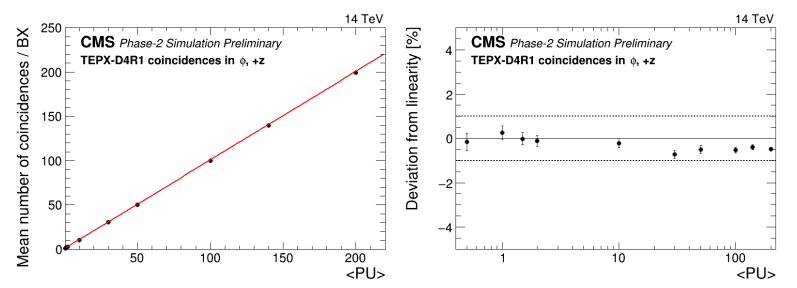
\includegraphics[width=0.6\columnwidth]{SP1.png}
  \caption{Left: Simulated mean number of coincidences in phi \& r for TEPX Disk 4 Ring 1 as a function of pileup. Right: Non-linearity is within 1 \% for entire pileup range. }
  \label{fig:CMS}
\end{figure}

\begin{table}[htb]
  \centering
   \caption{Expected statistical precision for Disk 4 Ring 1.}
  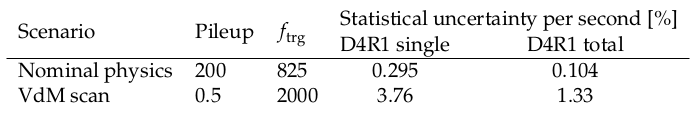
\includegraphics[width=0.6\columnwidth]{SP3.png}
  \label{fig:CMS}
\end{table}



\newpage
\section{BEAM INDUCED BACKGROUND MEASUREMENT USING D4R1}
Disk 4 Ring 1 (D4R1) will have dual purpose, luminosity and beam induced background (beam gas \& beam halo) measurements. It will be operated during LHC ramp when beams are not colliding for measuring beam induced backgrounds. First bunch in a train or noncolliding bunches will be used for
beam-induced background measurements. Beam induced backgrounds (BIB) will dominate out-of-time particles and albedo (afterglow) after at least 30 empty bunch crossings ($\approx$ 0.75 $\mu$ s). Incoming beam induced background will be separated from the first
collision products by about 17.8 ns at the position of D4R1. Fine timing system of D4R1 modules will be used so that incoming beam induced background will be seen one 25 ns clock cycle before the collision products to be clearly distinguished from collision products.
Optimization of efficiency is done by combining CMSSW BIB simulations with pileup simulation to extract time of flight vs deposited
charge distribution for BIB and collision hits. LHC clock is changing during ramp which will be handled by D4R1 trigger and timing system to operate D4R1 on LHC clock and not on CMS clock during ramp.


\begin{figure}[htb]
  \centering
  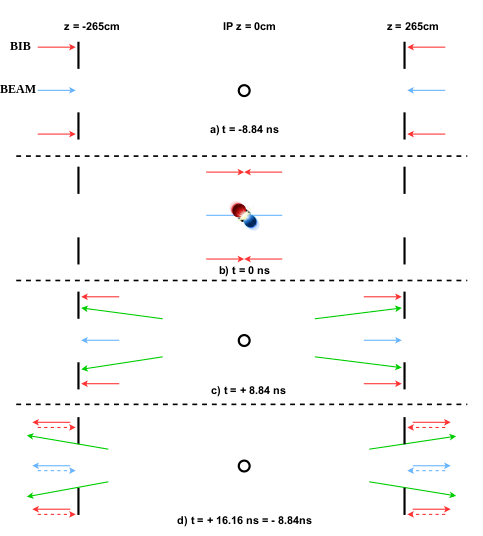
\includegraphics[width=0.4\columnwidth]{BIB.png}
  \caption{Basic principle of measuring beam-induced background with TEPX D4R1 at the beginning of a bunch train. }
  \label{fig:CMS}
\end{figure}

\begin{figure}[htb]
  \centering
  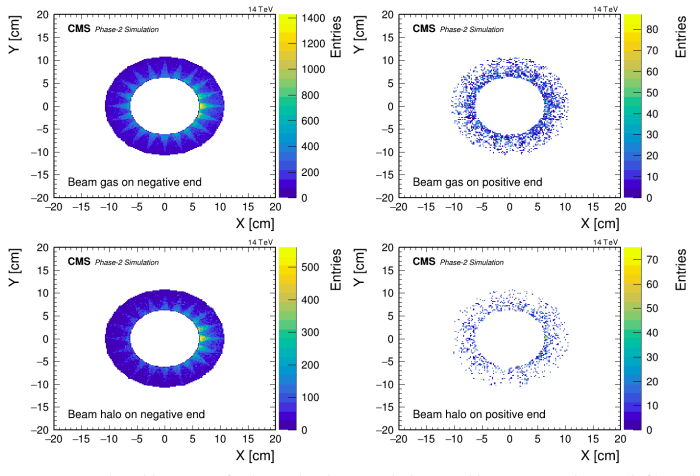
\includegraphics[width=0.5\columnwidth]{bib_new.png}
  \caption{Simulated beam-background hitmaps for D4R1 at the -z (left) and +z (right) end of CMS. The top row shows hits caused by the interactions of the primary protons with residual gas in the beam pipe along the LHC arcs (beam gas), while the lower row shows beam halo events, caused by off-orbit protons interacting with the collimators.}
  \label{fig:CMS}
\end{figure}


\section{Summary}
CMS detector will undergo several upgrades for High Luminosity (HL)-LHC era. It will have a new tracker with better radiation tolerance, increased granularity and extended pseudorapidity coverage. New tracker will be used for tracking, luminosity and beam induced background measurements. Luminosity measurement by TEPX will be based on real time pixel clusters or coincidences counting method on FPGA. Trigger and timing for luminosity measurement will be provided by a BRIL trigger board independent of CMS L1 triggers. TEPX luminosity processing will be performed by a separate luminosity processor board consisting of pixel clustering and histogramming instances to which the DTC backend will send data. Beam induced background measurement will be done by D4R1 utilizing first bunch in a train or noncolliding bunches and operating it on LHC clock and not on CMS clock during ramp. Linearity of TEPX luminometer is expected to be within 1\% over entire pileup range and statistical precision of 0.1\% at <PU>=200.


\begin{thebibliography}{99}
\bibitem{...}
CMS Collaboration, “The Phase-2 Upgrade of the CMS Beam Radiation
Instrumentation and Luminosity Detectors - Technical Design Report”.
CERN-LHCC-2021-008, CMS-TDR-023.
\bibitem{...}
CMS Collaboration, “The Phase-2 Upgrade of the CMS Beam Radiation,
Instrumentation, and Luminosity Detectors: Conceptual design”, CMS Public
Note CMS-NOTE-2019-008 (2020).
\bibitem{...}
CMS Collaboration, Precision luminosity measurement in proton-proton
collisions at 13 TeV in 2015 and 2016 at CMS, arXiv: 2104.01927.
\bibitem{...}
CMS Collaboration, CMS luminosity measurement for the 2017 data-taking
period at 13 TeV, CMS PAS LUM-17-004 (2018).
\bibitem{...}
CMS Collaboration , CMS luminosity measurement for the 2018 data-taking
period at 13 TeV, CMS PAS LUM-18-002 (2019).

\end{thebibliography}

\end{document}
